\chapter{Introduction}

\section{What is a Model of a System?}
A model is a simplified and approximate representation of a system, that allows reasoning on the systems properties. \textbf{So we construct models in order to understand some aspect of that system}. We include in the model only the aspect of the system that we consider essential, omitting details that would only complicate the analysis.

\subsection{Understanding the model}
After designing our model, then in order to acquire new knowledge, we have to \textbf{analyze the model} (like a child play with a toy to understand what it does), then we have to apply some \textbf{reasoning} regarding the result given during the analysis. 

\subsection{Errors}
All the three steps listed above (Modelling, Analysis, and Reasoning), \textbf{can be sources of errors}. The model can be too abstract; the analysis can be too inaccurate; or the interpretation itself could be wrong. \textbf{Recall that the result that you get are showing you only something about the real system, you need to generalise what the result means.}

\subsection{Examples of Models}

\subsubsection{Planimetries/project and scale models}
In architecture planimetries and scale models are used to assest structural properties at design time, in order to evaluate the result in advance.

\subsubsection{Life Science}
In biology rats (in-vivo model) or a cell colture (in-vitro model) are used as model for the human being. 

\subsubsection{In Silico Models}
In biology there are also computer-based techniques are usually faster and cheaper than in vivo e in vitro models. They simulate the interaction between proteins.

\subsection{Mathematical Models}
Mathematics provides tools for building abstract models of almost everything like \textbf{geometry} for Architecture or \textbf{differential equations} for Weather. Mathematical models have two advantages:

\begin{itemize}

\item They are formal model specification languages, meaning it is not an ambiguous model.

\item there are a lot of analytical and numerical methods to analyze model of this type.

\end{itemize}

\subsection{Computational Models}
Computational Models is similar to Mathematical Models. A Computational Model is a mathematical representation of a dynamical system (systems which evolves over time) taking a computer-executable form.
\par in Computational Model we are restricting the class of systems of interest to dynamical systems (systems which evolve over time). 

\subsubsection{Dynamical Systems}
Dynamical systems are systems that \textbf{evolve} by changing their state over time. Typically the state of a dynamical system is represented by a finite set of variables called \textbf{state variables}. In addition we will have some some law/rules/equations that describe how the state variables will vary over time. Our focus will be in prediction or analyze how the state of a dynamic system changes.
\par There are different types of dynamical systems depending on how the values of the variables change in either a discrete or a continuous way (or both).
\par \textbf{Note: time can be interpreted as a discrete or continuous entity}. 

\begin{figure}[h]
    \centering
    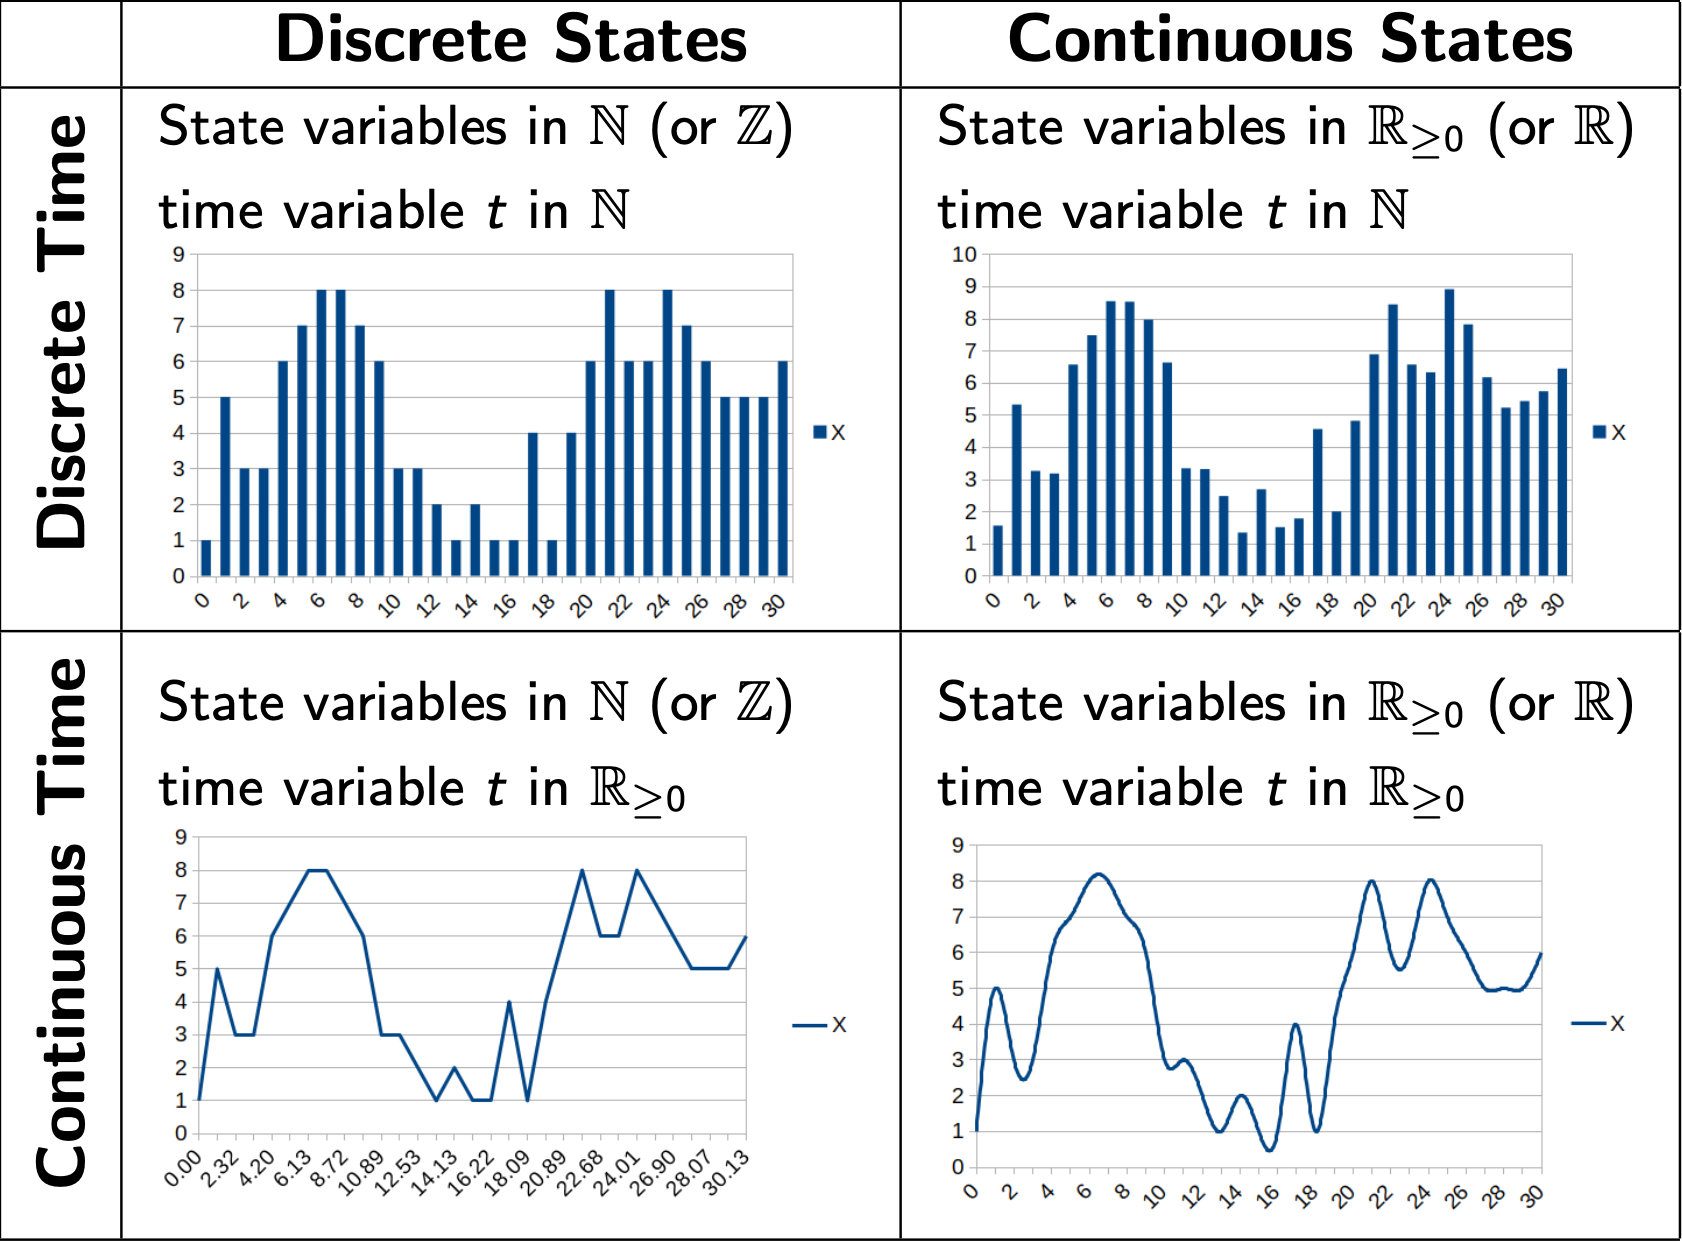
\includegraphics[width=0.8\textwidth]{Images/01-Introduction/states.png}
    \caption{All possible types of dynamical systems.}
\end{figure}

\subsection{Case of application}
What kind of analysis could we do with models of dynamical systems?

\begin{itemize}
    \item \textbf{Reachability of states:} predict the future state of the dynamical system.

    \item \textbf{Behavioral patterns:} the sequence of state that I pass through over time.

    \item \textbf{Effects of perturbations/ control strategies:} once I have a model of a system and I can simulate it, I can try to study how it will behave if I modify it.
\end{itemize}

\subsection{How to build a computational models?}
There are multiple ways

\subsubsection{The Data-driven way}
The Data-driven way (e.g. machine learning) consist in starting from the data of the system you want to model and then you apply some machine learning/optimization/whatever method to infer the model automatically. The generated model takes a form suitable for the inference method used. If enough data in available, it often works very well (good predictions), however inferred models are often very difficult to be interpreted (meaning that we can do good prediction, but we can't explain why they are correct).

\subsubsection{The Knowledge-driven way} (also called mechanistic models) consist in trying to reproduce through a mathematical model the internal mechanism of the system in order to reproduce the behaviour and to understand the internals of the systems. It requires limited data, but a good knowledge about the system functioning. Model construction usually requires some effort, and often predictions suffer from approximations but the method generated works also when few data are available; the model is interpretable: it contributes to understanding why a system behaves as observed; modelling allows validation hypotheses on the system functioning.

\section{What is a complex system?}
A complex system is a system consisting of many components (typically with a simple individual behaviours) interacting with each other, from these interaction emerges the global behaviour of the system.

\subsubsection{Complex Networks}
Complex Networks is a graph with complex structural properties. The dynamics of these networks and its evolution is a field of study (complex networks theory).

\subsection{Modeling notations for complex systems}
Many modeling languages are available for complex systems:

\begin{itemize}
    \item \textbf{mathematics:} Recurrence relations and differential equations.

    \item \textbf{concurrency theory:} we can apply methods seen in the study of concurrent system like Petri nets. Rewrite rules (Multiset rewriting) that describe the different events that happens in a complex systems as rules.

    \item \textbf{artificial life:} approaches proposed to try to reproduce behaviour seen in life. Cellular automata that describe the population as a grid; agents based model in which you explicit as an agent (e.g. an algorithm or set of functions/procedures) and then you can put the agent in a virtual environment to see how they behave together. 
\end{itemize}

\section{Analyze the model}
Modeling languages allow the modeler to express relationships between the state variables of a system and the rules/laws that determine the change of their values over time. The dynamics (or behaviour) of the systems (the actual sequences of states reached by the system over time) can be computed according to the semantics of the modeling language.

\section{Analyze the behaviour}
After the model has been specified, then there are multiple way to analyze the model. 

\subsection{Simulation}
You can try to apply some simulation algorithm in order to try to execute that model to have a possible evolution of the system. If the system is deterministic you have only one possible evolution, instead if the system is stochastic-probabilistic you will repeat the simulation several time and get different behaviour of the system. \textbf{So simulations can give you only some possible behaviour, not all}. Instead of running simulations to construct some description of the overall behaviour of the systems, it can be done by using \textbf{transition systems}. 

\subsubsection{Transition system}
A transition system is a graph (possible infinite) that describe the possible behaviour of a system. A possible transition system is the \textit{Makov chain}

\subsection{Model Checking}
It is an approach that determine whether the whole transition system satisfies a given dynamical property.

\section{Modeling vs programming}
The approach that we will follow to analyze dynamical systems is similar to the approach used to analyze programs

\begin{figure}[h]
    \centering
    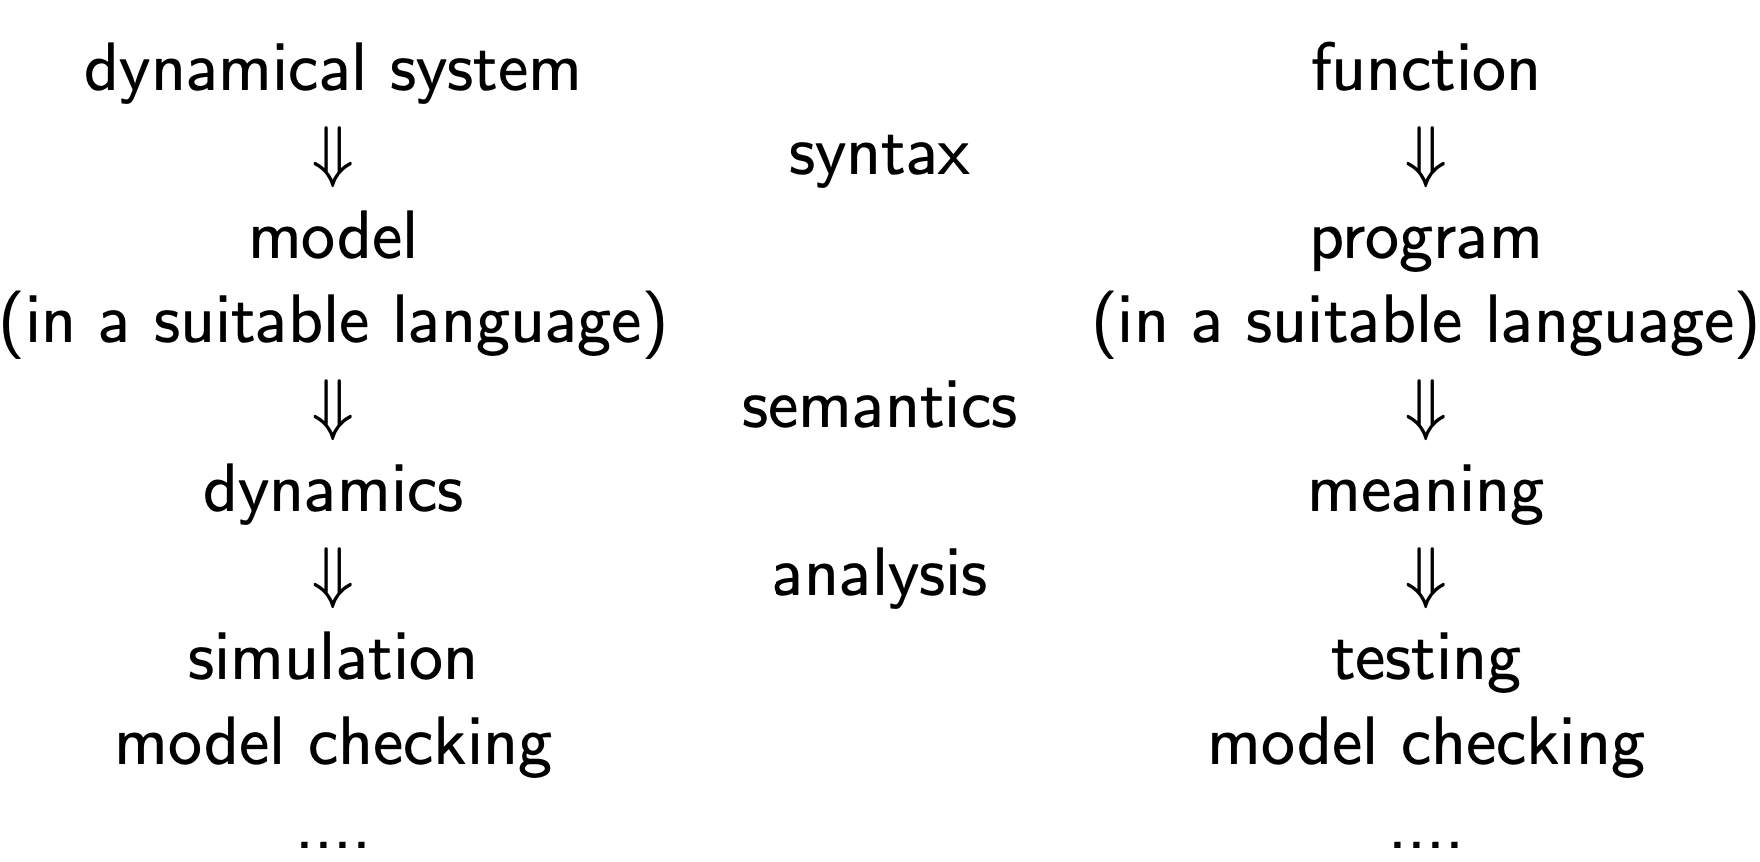
\includegraphics[width=0.9\textwidth]{Images/01-Introduction/model vs programming.png}
    \caption{Modeling vs programming.}
\end{figure}
